\newcommand{\vigenereFigFrom}{
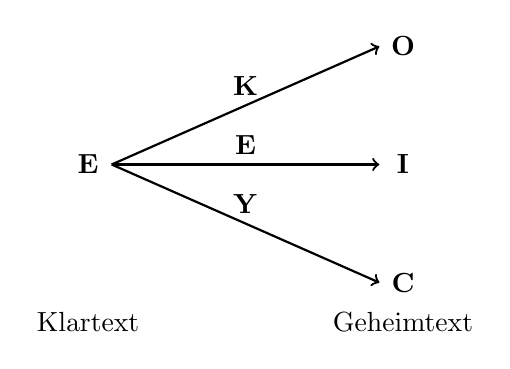
\begin{tikzpicture}
 % Klartext und Geheimtext Labels
 \node at (0, 0) {\textbf{E}};
 \node at (4, 1.5) {\textbf{O}};
 \node at (4, 0) {\textbf{I}};
 \node at (4, -1.5) {\textbf{C}};

 % Verbindungspfeile mit Schlüsseln
 \draw[->, thick] (0.3, 0) -- (3.7, 1.5) node[midway, above] {\textbf{K}};
 \draw[->, thick] (0.3, 0) -- (3.7, 0) node[midway, above] {\textbf{E}};
 \draw[->, thick] (0.3, 0) -- (3.7, -1.5) node[midway, above] {\textbf{Y}};

 % Labels Klartext und Geheimtext
 \node[align=center] at (0, -2) {Klartext};
 \node[align=center] at (4, -2) {Geheimtext};
\end{tikzpicture}
}

\newcommand{\vigenereFigTo}{
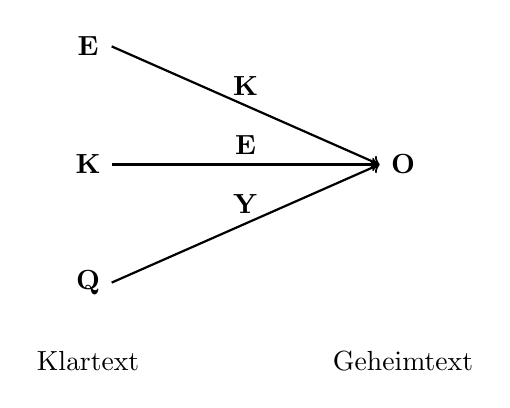
\begin{tikzpicture}
 % Klartext letters
 \node at (0, 1.5) {\textbf{E}};
 \node at (0, 0) {\textbf{K}};
 \node at (0, -1.5) {\textbf{Q}};
 
 % Geheimtext letter
 \node at (4, 0) {\textbf{O}};
 
 % Verbindungspfeile mit Schlüsseln
 \draw[->, thick] (0.3, 1.5) -- (3.7, 0) node[midway, above] {\textbf{K}};
 \draw[->, thick] (0.3, 0) -- (3.7, 0) node[midway, above] {\textbf{E}};
 \draw[->, thick] (0.3, -1.5) -- (3.7, 0) node[midway, above] {\textbf{Y}};
 
 % Labels Klartext und Geheimtext
 \node[align=center] at (0, -2.5) {Klartext};
 \node[align=center] at (4, -2.5) {Geheimtext};
\end{tikzpicture}
}

\newcommand{\vigenereFig}{
\begin{figure}[H]
	\centering
	\begin{subfigure}{.35\textwidth}
	\centering
	\resizebox{\textwidth}{!}{
	\vigenereFigFrom
	}
	\end{subfigure}
	\begin{subfigure}{.35\textwidth}
	\centering
	\resizebox{\textwidth}{!}{
	\vigenereFigTo}
	\end{subfigure}
	\end{figure}
	}
	
% Caesar dial, cleartext inside, cryptotext outside
\newcommand\caesar[1][3]{%
  \begin{tikzpicture}
    \def\r{2}
    \def\dr{0.5}
    \def\ri{1.4}
    \def\dri{0.5}
    \def\rotate{#1}%% number of shifts
    \coordinate (origin) at (0,0);
    \draw[fill=gray!60] (origin) circle (1pt);
    \draw (origin) circle (\r);
    \draw (origin) circle (\r+\dr);
    \draw (origin) circle (\ri);
    \draw (origin) circle (\ri+\dri);
    \foreach \letter [count=\ind from 0,evaluate=\ind as \ang using 90-\ind*360/26] in {A,B,...,Z}{%
        \node[rotate={\ang-90}] at ($(origin)+(\ang:{\r+\dr/2})$) {\textcolor{RoyalBlue}{\letter}};
        \draw({\ang+0.5*360/26}:\r)--({\ang+0.5*360/26}:\r+\dr);
      }
    \foreach \letter [count=\ind from 0,evaluate=\ind as \ang using 90-\ind*360/26-\rotate*360/26] in {A,B,...,Z}{%
        \node[rotate={\ang-90}] at ($(origin)+(\ang:{\ri+\dri/2})$) {\textcolor{ForestGreen}{\letter}};
        \draw({\ang+0.5*360/26}:\ri)--({\ang+0.5*360/26}:\ri+\dri);
      }
      \ifnumequal{\rotate}{0}{}{
      \draw[-latex] (90:\ri-0.3) arc (90:{90-\rotate*360/26}:\ri-0.3)node[pos=0.5,anchor=90-\rotate*180/26]{$\rotate$};}
    
  \end{tikzpicture}
}

% Caesar dial, cleartext outside, cryptotext inside
\newcommand\caesarreverse[1][3]{%
  \begin{tikzpicture}
    \def\r{2}
    \def\dr{0.5}
    \def\ri{1.4}
    \def\dri{0.5}
    \def\rotate{#1}%% number of shifts
    \coordinate (origin) at (0,0);
    \draw[fill=gray!60] (origin) circle (1pt);
    \draw (origin) circle (\r);
    \draw (origin) circle (\r+\dr);
    \draw (origin) circle (\ri);
    \draw (origin) circle (\ri+\dri);
    % Klartext AUSSEN (grün)
    \foreach \letter [count=\ind from 0, evaluate=\ind as \ang using 90-\ind*360/26-\rotate*360/26] in {A,B,...,Z}{%
        \node[rotate={\ang-90}] at ($(origin)+(\ang:{\r+\dr/2})$) {\textcolor{ForestGreen}{\letter}};
        \draw({\ang+0.5*360/26}:\r)--({\ang+0.5*360/26}:\r+\dr);
      }
    % Geheimtext INNEN (blau)
    \foreach \letter [count=\ind from 0, evaluate=\ind as \ang using 90-\ind*360/26] in {A,B,...,Z}{%
        \node[rotate={\ang-90}] at ($(origin)+(\ang:{\ri+\dri/2})$) {\textcolor{RoyalBlue}{\letter}};
        \draw({\ang+0.5*360/26}:\ri)--({\ang+0.5*360/26}:\ri+\dri);
      }
    % Pfeil AUSSEN mit Text OBEN
    \ifnumequal{\rotate}{0}{}{
      \draw[-latex] 
        (90:\r+\dr+0.3) 
        arc[start angle=90, end angle={90-\rotate*360/26}, radius=\r+\dr+0.3]
        node[midway, yshift=8pt] {$\rotate$};
    }
    
  \end{tikzpicture}
}


% code to generate a figure illustrating monoalphabetic substitution for a given substitution alphabet (first argument)
\newcommand{\multiKey}[1]{
\resizebox{\textwidth}{!}{
\begin{tikzpicture}[node distance=0.5cm and 0.5cm]
	\node(topL) at (-1,1.5) {};
	\node(bottomL) at (-1,0) {};
    % Erste Reihe (oberes Alphabet) automatisch generiert
    \foreach \i [count=\j from 1] in {A,...,Z} {
        \node (top\j) at (\j, 1.5) {\i};
    }

    % Zweite Reihe (unteres Alphabet) basierend auf dem Argument
    \foreach \i [count=\j from 1] in {#1} {
        \node (bottom\j) at (\j, 0) {\i};
    }

    % Verbindungen
    \foreach \i in {1,...,26} {
        \draw[<->] (top\i) -- (bottom\i);
    }
    
    % Zweiter Pfeil von bottomL nach topL, um 0.1cm nach rechts verschoben
    \draw[->,red,ultra thick] ($(bottomL.north)+(.5cm,0)$) -- node[right]{\emoji{key}}($(topL.south)+(.5cm,0)$);
    
    \draw[->,red,ultra thick] (topL) -- node[left]{\emoji{lock}} (bottomL);

\end{tikzpicture}
}
}

\begin{frame}[fragile]{Häufigkeitsverteilung}
		\begin{figure}[H]
			\centering
			\multiKey{Z,E,A,B,C,D,Y,X,W,H,I,V,U,T,G,F,J,K,R,Q,L,M,S,N,P,O}
			$\rightarrow$ \textbf{Wie knacken wir so etwas?}
		\end{figure}
\end{frame}

\begin{frame}[fragile, label=hauefigkeit]{Häufigkeitsverteilung}
	\begin{multicols}{2}
		    \begin{figure}[H]
			\centering
			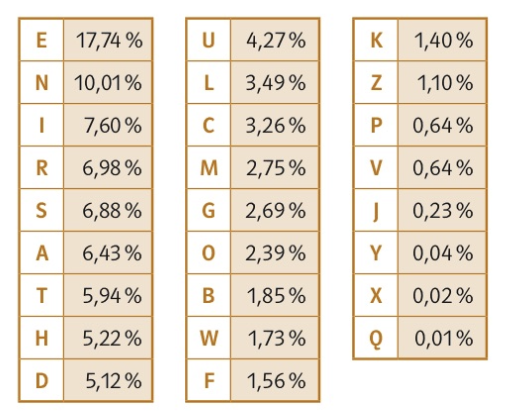
\includegraphics[width=\linewidth]{GrundlagenInfo/03_Kryptologie/Figures/freq.png}
		\end{figure}
		\columnbreak
		\[h_\square (T)\]
		= Häufigkeit von Buchstabe $\square$ in Text $T$.
	\end{multicols}
    \begin{figure}[H]
    	\centering
    	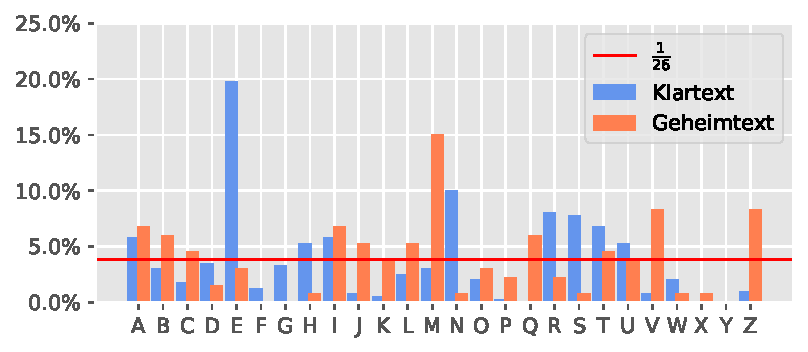
\includegraphics[width=.7\textwidth]{GrundlagenInfo/03_Kryptologie/Figures/letterfreq_end_dec0}
    \end{figure}
\end{frame}


\begin{frame}[fragile]{Häufigkeitsanalyse}
\textbf{Problem}: Alle \textbf{monoalphabetischen} Kryptosysteme lassen sich mit einfacher Häufigkeitsanalyse knacken
    \begin{figure}[H]
        \centering
        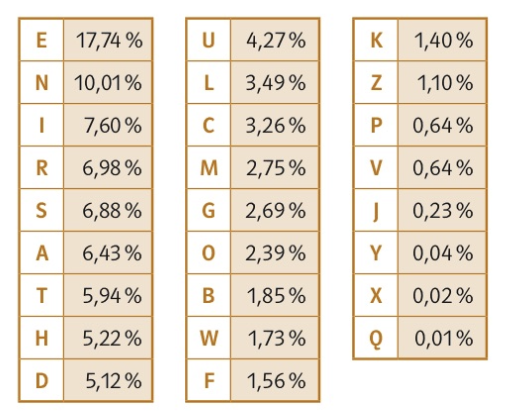
\includegraphics[width=.5\linewidth]{GrundlagenInfo/03_Kryptologie/Figures/freq.png}
        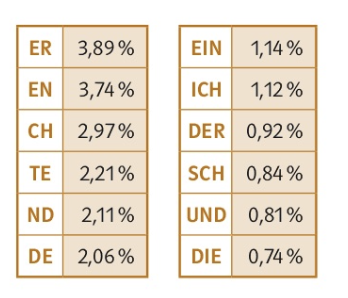
\includegraphics[width=.35\linewidth]{GrundlagenInfo/03_Kryptologie/Figures/bigramme.png}
    \end{figure}
    %\textcolor{red}{\rule{\textwidth}{.3mm}}\\[-.1cm]
    \defverbatim{\verbOne}{
    \small\begin{verbatim}
MUMMUXJUQYMHQOUSUTUQNGWTJQVHUMXQUXQJSUVYPPUM
--------------------------------------------
    \end{verbatim}
    U kommt 10-mal vor, M kommt 6-mal vor, Q kommt 6-mal vor}
    \defverbatim{\verbTwo}{
    \small\begin{verbatim}
MUMMUXJUQYMHQOUSUTUQNGWTJQVHUMXQUXQJSUVYPPUM
NENNE--EI-N-I-E-E-EI-----I--EN-IE-I--E----EN
    \end{verbatim}
    U=E, M=N, Q=I?
    }
    \defverbatim{\verbThree}{
    \small\begin{verbatim}
MUMMUXJUQYMHQOUSUTUQNGWTJQVHUMXQUXQJSUVYPPUM
NENNED-EI-N-I-E-E-EI-----I--ENDIEDI--E----EN
\end{verbatim}
Wir fahren nun mit Trigrammen weiter: ``Die''?}
    \defverbatim{\verbFour}{
    \small\begin{verbatim}
MUMMUXJUQYMHQOUSUTUQNGWTJQVHUMXQUXQJSUVYPPUM
NENNEDREI-N-I-E-E-EI----RI--ENDIEDIR-E----EN
\end{verbatim}
``D-EI''=``Drei''?}
    \defverbatim{\verbFive}{
    \small\begin{verbatim}
MUMMU|XJUQ|YMHQOUSUTUQNGWTJQVHUM|XQU|XQJ|SUVYPPUM
NENNE|DREI|-N-I-E-E-EI----RI--EN|DIE|DIR|-E----EN
\end{verbatim}
	Man beginnt einzelne Wörter zu erkennen...
    }
    \defverbatim{\verbSix}{
    \small\begin{verbatim}
MUMMU|XJUQ|YMHQOU|SUTUQNGWTJQVHUM|XQU|XQJ|SUVYPPUM
NENNE|DREI|ANTIKE|GEHEIMSCHRIFTEN|DIE|DIR|GEFALLEN
    \end{verbatim}
    \emoji{blush}
    }
    \only<1>{\verbOne}
    \only<2>{\verbTwo}
    \only<3>{\verbThree}
    \only<4>{\verbFour}
    \only<5>{\verbFive}
    \only<6>{\verbSix}
\end{frame}

\begin{frame}{Auftrag}
Skript
\begin{itemize}
   \item \aufgabebox{1.9}
   \item \challengebox{1.10, 1.11}
\end{itemize}
\end{frame}

\begin{frame}{Mono- und Polyalphabetische Kryptosysteme}
	\begin{itemize}[<+->]
		\item \textbf{Monoalphabetisch}: Jeder Buchstabe wird immer durch denselben Buchstaben erstetzt, unabhängig von seiner Position im Klartext. \textbf{Nachteil}: Einfache Entschlüsselung durch Häufigkeitsanalyse
		\item \textbf{Polyalphabetisch}: Jeder Buchstabe kann durch unterschiedliche Buchstaben ersetzt werden
	\end{itemize}
\end{frame}

%\begin{frame}{Kerkhoffs'sches Prinzip der Sicherheit}
%	\begin{center}
%		``Ein Kryptosystem ist \textbf{sicher}, wenn das Kryptosystem [= der Algorithmus] öffentlich bekannt ist und es trotzdem ohne die Kenntnis des verwendeten Schlüssels nicht möglich ist, aus einem Geheimtext den ursprünglichen Klartext abzuleiten.''
%	\end{center}    
%\end{frame}